
%%%%%%%%%%%%%%%%%%%%%%%%%%%%%%%%%%%%%%%%%%%%%%%%%%%%%%%%%%%%%%%%%%%%%%%%%%%%%%%
%%%% Begin of Document
%%%%%%%%%%%%%%%%%%%%%%%%%%%%%%%%%%%%%%%%%%%%%%%%%%%%%%%%%%%%%%%%%%%%%%%%%%%%%%%
\DeclareRobustCommand{\diag3}[3]{
	\left(
		\begin{matrix}
		#1	& 0  		& \cdots	 & 0 \\
		0 	& \ddots	& \ddots 	 & \vdots \\
		\vdots 	& \ddots 	& \ddots 	 & 0 \\
		0 	& \cdots        & 0		 & #3\\
		\end{matrix}
	\right) 
}
\DeclareRobustCommand{\triang2}[2]{
	\left(
		\begin{matrix}
		#1_{1,1}#2	& 0 		& \cdots	 & 0 \\
		\vdots	 	& \ddots	& \ddots 	 & \vdots \\
		\vdots 		& 	 	& \ddots 	 & 0 \\
		#1_{n,1}#2	& \cdots        & \cdots	 & #1_{n,n}#2\\
		\end{matrix}
	\right) 
}
\DeclareRobustCommand{\figref}[1]{\mbox{ Fig. \ref{#1}}}
\DeclareRobustCommand{\defref}[1]{\mbox{ Definition \ref{#1}}}
\DeclareRobustCommand{\enumref}[1]{\mbox{\ref{#1}}}
\DeclareRobustCommand{\appendixref}[1]{\mbox{ Appendix \ref{#1}}}
\DeclareRobustCommand{\tupelref}[2]{\mbox{\enumref{#1} \enumref{#2}}}
\DeclareRobustCommand{\eqref}[1]{\mbox{ (\ref{#1})}}
\DeclareRobustCommand{\carlos}[1]{{\color{green} Carlos #1}}
\DeclareRobustCommand{\citeme851}{({\color{red} control theory lecture, the guy has not replied yet for a better citation)}}
%
\definecolor{lightblue}{rgb}{.187,.613,.594}
%%\definecolor{lightblue}{rgb}{0.145,0.6666,1}
%
%
\hyphenation{resolution occlusions}
%  % Eye Catcher
%  {
\includegraphics[heightm4.5em]{../../../../../../Administration/Logos/EmmyNoether}
%  } 
%  % Title
%  {Application of Input to State Stability to ecological reservoir models}
%  % Authors
%  {
% {\bf  Markus M\"uller, Carlos A. Sierra}   \\
%  {\small  <csierra@bgc-jena.mpg.de> } %\\ 
%%  Independent Research Group \\
%%  Theoretical Ecosystem Ecology
%  }
%  % University logo
%  {% The makebox allows the title to flow into the logo, this is a hack because of the L shaped logo.
%%   
\includegraphics[height=5em]{Minerva} \\
%   
\includegraphics[height=2em]{BGClogo}
%  }
%
%%%%%%%%%%%%%%%%%%%%%%%%%%%%%%%%%%%%%%%%%%%%%%%%%%%%%%%%%%%%%%%%%%%%%%%%%%%%%%%
%%%% Now define the boxes that make up the poster
%%%%---------------------------------------------------------------------------
%%%% Each box has a name and can be placed absolutely or relatively.
%%%% The only inconvenience is that you can only specify a relative position 
%%%% towards an already declared box. So if you have a box attached to the 
%%%% bottom, one to the top and a third one which should be in between, you 
%%%% have to specify the top and bottom boxes before you specify the middle 
%%%% box.
%%%%%%%%%%%%%%%%%%%%%%%%%%%%%%%%%%%%%%%%%%%%%%%%%%%%%%%%%%%%%%%%%%%%%%%%%%%%%%%
%    %
%
%%%%%%%%%%%%%%%%%%%%%%%%%%%%%%%%%%%%%%%%%%%%%%%%%%%%%%%%%%%%%%%%%%%%%%%%%%%%%%%
%\headerbox{Challenge}{name=Challenge,span=2,column=0, row=0 }{
%  %%%%%%%%%%%%%%%%%%%%%%%%%%%%%%%%%%%%%%%%%%%%%%%%%%%%%%%%%%%%%%%%%%%%%%%%%%%%%%
%\smaller% \centering
%\noindent
%Many models in ecology and biogeochemistry, in particular models of the global
%carbon cycle, can be generalized as systems of non-autonomous ordinary
%differential equations (ODEs). For many applications, it is important to
%determine the stability properties for this type of systems, but most methods
%available for autonomous systems are not necessarily applicable for the
%non-autonomous case.  We discuss here stability notions for non-autonomous
%nonlinear models represented by systems of ODEs explicitly dependent on time
%and a time-varying input signal.  
%Is there a stability concept that is:
%\begin{enumerate}
%	\item
%	broad enough to encompass these models
%	\item
%	rigorous enough to be proved analytically 
%	\item
%	interpretable in ecologically meaningful terms ?
%\end{enumerate}
%}
%%%%%%%%%%%%%%%%%%%%%%%%%%%%%%%%%%%%%%%%%%%%%%%%%%%%%%%%%%%%%%%%%%%%%%%%%%%%%%%
%\headerbox{Example: general soil model}{name=general,span=2,column=0, row=2, below=Challenge}{
%  %%%%%%%%%%%%%%%%%%%%%%%%%%%%%%%%%%%%%%%%%%%%%%%%%%%%%%%%%%%%%%%%%%%%%%%%%%%%%%
%\smaller %\centering
%\begin{multicols}{2}
%    		\[
%		\mathbf{\dot{C}}= \bm{I}(t) + {\bf T}(\mathbf{C},t) \cdot {\bf N}(t, \bm{C}) \cdot \bm{C}(t)
%    		\]
%    		\begin{equation*}	
%    		\label{structCond}
%    		\begin{array}{lcl}	
%    		N_{i,i}(\mathbf{C},t) 		&\ge& 	 0 \quad \forall i \\
%    		T_{i,i}(\mathbf{C},t) 		&=& 	 -1 \quad \forall i \\
%    		T_{i,j}(\mathbf{C},t) 		&\ge& 	 0 \quad \forall i \ne j \\
%    		\sum_i T_{i,j}(\mathbf{C},t) 	&=  &	 1\quad \forall j 
%    		\end{array}	
%    		\end{equation*}	
%    		This model structure generalizes most SOM decomposition models with any arbitrary number of pools, including those describing nonlinear interactions among state variables. It enforces mass balance and substrate dependence of decomposition, and it is flexible enough to describe:
%		\begin{enumerate}
%		\item Heterogeneity of decomposition rates
%		\item Transformations of organic matter
%		\item Environmental variability effects
%		\item Organic matter interactions
%		\end{enumerate}
%
%		Examples for nonlinear models are:
%		\begin{enumerate}
%			\item Exoenzyme models \citep{Schimel,Sinsabaugh}
%			\item AWB \citep{Allison}
%			\item Bacwave \citep{Zelenev}
%			\item MEND \citep{WangMEND}
%			\item Manzoni \citep{Manzoni07}
%		\end{enumerate}
%		Also linear models fit into the general framework 
%		\begin{enumerate}
%			\item Henin's model \citep{HeninDupuis, Henin}
%			\item ICBM \citep{AndrenKatterer}
%			\item RothC \citep{Jenkinson, Coleman} 
%			\item Century \citep{Parton} 
%			\item Fontaine 1-4 \citep{Fontaine}
%		\end{enumerate}
%		One general concept to encompass especially  these nonlinear  models is clearly desirable.
%
%
%
%\end{multicols}
%}
%%%%%%%%%%%%%%%%%%%%%%%%%%%%%%%%%%%%%%%%%%%%%%%%%%%%%%%%%%%%%%%%%%%%%%%%%%%%%%%
%\headerbox{Results I, ISS as generalization of available stability concepts }{name=generalsoilmodel,span=2,column=0, row=2, below=general}{
%  %%%%%%%%%%%%%%%%%%%%%%%%%%%%%%%%%%%%%%%%%%%%%%%%%%%%%%%%%%%%%%%%%%%%%%%%%%%%%%
%\begin{multicols}{2}
%\smaller %\centering
%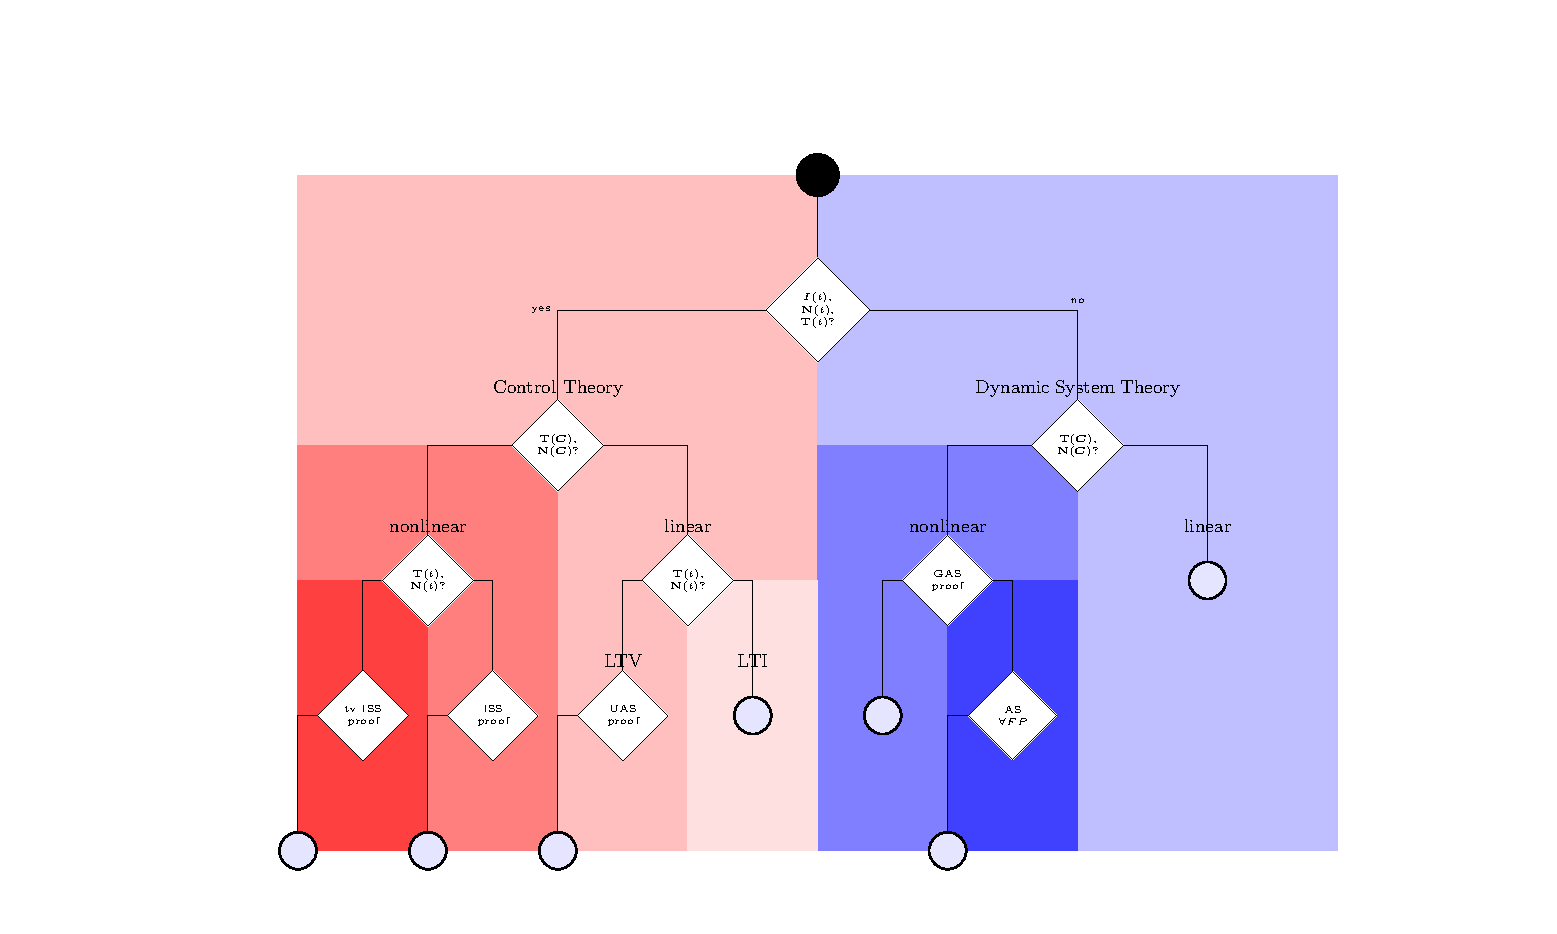
\includegraphics[width=\columnwidth,clip=true,trim=4.5cm 1cm 1cm 1cm]{Fig1.pdf}
%
%\columnbreak
%\noindent
%The graph shows different stability concepts one could try to establish for the
%general soil model mentioned above depending on properties of its components 
%$\mathbf{I},\mathbf{T}$ and $ \mathbf{N}$. The hardest to prove is Input to
%State Stability for time varying systems (ISStv) in the lower left corner.  It
%turns out that ISStv also generalizes all the other concepts mentioned:
%\begin{itemize}
%\item 
%In the case of Linear Time Invariant (LTI) systems  ISS follows from the properties of the matrix.(eigenvalues)
%\item 
%In the case of Linear Time Variant (LTV) systems it can be established if sufficient information about the 
%state transition operator allows to prove uniform asymptotic stability UAS.
%\item
%For input free system (on the blue right-hand side) ISS reduces to Global Asymptotic Stability (GAS)
%\item
%\dots
%
%\end{itemize}
%\end{multicols}
%}
%%%%%%%%%%%%%%%%%%%%%%%%%%%%%%%%%%%%%%%%%%%%%%%%%%%%%%%%%%%%%%%%%%%%%%%%%%%%%%%
%  \headerbox{Results II, ISS like behavior and proof for example system}{name=combi,column=2,span=2, row=0}{
%%%%%%%%%%%%%%%%%%%%%%%%%%%%%%%%%%%%%%%%%%%%%%%%%%%%%%%%%%%%%%%%%%%%%%%%%%%%%%%
%\smaller %\centering
%\begin{multicols}{2}
%The graphs show the reactions of a prototypical class of nonlinear two pool soil models to a disturbing time varying signal. 
%This model is a technically simple place holder for ecologically motivated nonlinear systems like the soil models mentioned above to be analyzed in the future. It is given by:\\
%\begin{eqnarray}
%\dot{C}_x=I_{x}(t)  - \left(C_{x}^{2} + C_{x}\right) \operatorname{k_{x}}{\left (t \right )}\\
%\dot{C}_y=I_{y}(t)  - \left(C_{y}^{2} + C_{y}\right) \operatorname{k_{y}}{\left (t \right )}
%\end{eqnarray}
%where $C_x,C_y$ are the carbon contents of two unconnected pools and the bounded  periodic functions $k_x(t) $ and $k_y(t) $ with:\\ 
%\begin{eqnarray}
%k_{x_{min}}\le  k_x(t) \le k_{x_{max}} \\k_{y_{min}} \le  k_y(t) \le k_{y_{max}}
%\end{eqnarray}
%describe the seasonal changes in decomposition speed.
%e.g.:\\ 
%\begin{eqnarray}
%k_x=\frac{k_{xmax}}{2} + \frac{k_{xmin}}{2} + \frac{1}{2} \left(k_{xmax} - k_{xmin}\right) \sin{\left (4 t \right )}\\k_y=\frac{k_{ymax}}{2} + \frac{k_{ymin}}{2} + \frac{1}{2} \left(k_{ymax} - k_{ymin}\right) \sin{\left (4 t \right )}
%\end{eqnarray}
%The system can have a fixed point: 
%$$ \mathbf{C}_f= \begin{pmatrix} C_{fx} \\ C_{fy} \end{pmatrix} $$
%if the input streams have the same period and phase as the decomposition rates. For constant input streams it stays in a predictable region (an invariant set in the phase plane) \\ 
%%\begin{eqnarray}
%%\mathbf{I}_0(t)=\left(\begin{matrix}\left(C_{fx}^{2} + C_{fx}\right) \operatorname{k_{x}}{\left (t \right )}\\\left(C_{fy}^{2} + C_{fy}\right) \operatorname{k_{y}}{\left (t \right )}\end{matrix}\right)
%%\end{eqnarray}
%%The fixpoint would be.
%%\[
%%\mathcal{A}=\{\mathbf{C}_f\}
%%\]
%%We will now disturb both mass influxes individually by perturbations $u_x(t),u_y(t)$ and get: 
%%\begin{eqnarray}
%%\dot{C}_x=I_{0 x}(t) + u_{x}(t) - \left(C_{x}^{2} + C_{x}\right) \operatorname{k_{x}}{\left (t \right )}\\
%%\dot{C}_y=I_{0 y}(t) + u_{y}(t) - \left(C_{y}^{2} + C_{y}\right) \operatorname{k_{y}}{\left (t \right )}
%%\end{eqnarray}
%The plots show the typical behavior of an ISS system: The changes in the state variables will asymptotically converge to a region of stability around an invariant set, whose size is a monotone function of the size of the disturbance (denoted by $|u|_{\infty}$).
%For this particular system we proved the ISS property rigorously. The proof relies on the construction of an ISS Lyapunov function whose choice is \emph{not determined but  inspired} by a property of the system interpretable in ecologically terms. Expressed casually: "The  system can counteract supply changes fast enough".
%This situation seems to be typical: The problem of establishing ISS for e.g. all the $\mathbf{I},\mathbf{T},\mathbf{N}$ models based on the ecologic principles they follow , is too hard.
%But bio-chemical of biophysical restrictions could provide clues to ISS proofs for a particular system.
%\\
%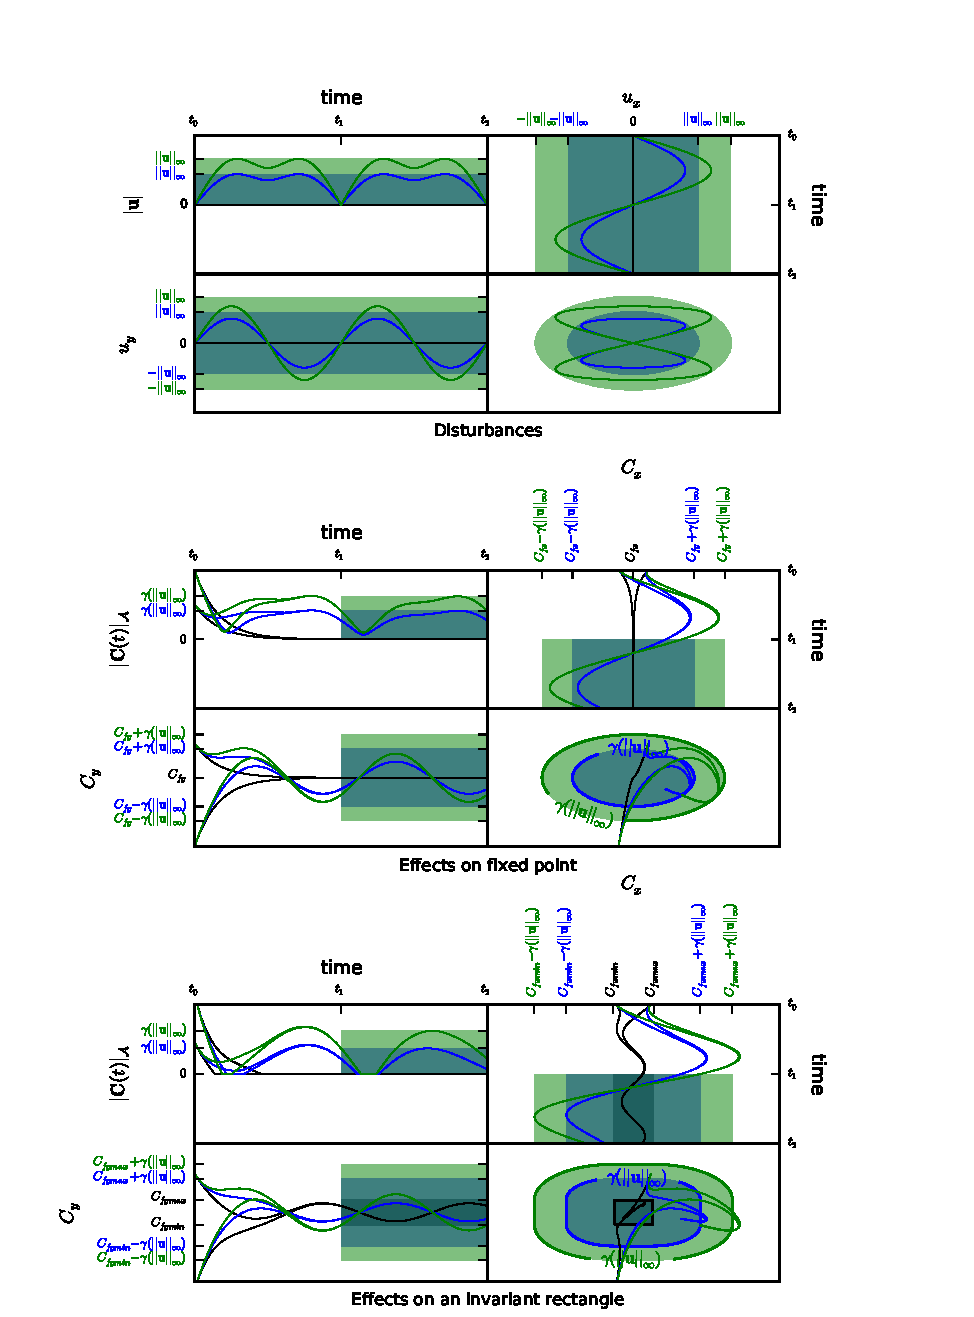
\includegraphics[width=\columnwidth]{combiPlot2.pdf}
%\\
%\begin{enumerate}
%	\item
%	The four plots on the top show the disturbances.
%	\item
%	The next four plots in the middle show the effect of this disturbances on the solutions for a system with fixed point. 
%	\item
%	The next four plots in the middle show the effect of this disturbances on the solutions for the system which no longer has a fixed point, but at least an invariant set, the dark blue square in the middle.
%\end{enumerate}
%\end{multicols}
%}
%%%%%%%%%%%%%%%%%%%%%%%%%%%%%%%%%%%%%%%%%%%%%%%%%%%%%%%%%%%%%%%%%%%%%%%%%%%%%%%
%\headerbox{Conclusion}{name=Intro,span=2,column=2, below=combi  }{
%\smaller %\centering
%%%%%%%%%%%%%%%%%%%%%%%%%%%%%%%%%%%%%%%%%%%%%%%%%%%%%%%%%%%%%%%%%%%%%%%%%%%%%%%
%\noindent
%We propose Input to State Stability (ISS) as
%candidate for the necessary generalization of the established analysis with
%respect to equilibria or invariant sets for autonomous systems, and showed for example systems its
%usefulness by applying it to reservoir models typical for element cycling in
%ecosystem, e.g. in soil organic matter decomposition.  In a forthcoming paper we  also showed how ISS
%generalizes existent concepts formerly only available for Linear Time Invariant
%(LTI) and Linear Time Variant (LTV) systems to the nonlinear case. 
%}
%
%%%%%%%%%%%%%%%
%%%%%%%%%%%
%\end{poster}
%\bibliography{GeneralModel}
%\bibliographystyle{abbrvnat}
%\end{document}
